\subsection{Metody redukcji wielowymiarowości}

Redukcja wymiaru często jest pośrednim etapem w zagadnieniu klasyfikacji, analizy skupień czy regresji. W określonych sytuacjach pozwala na poprawę skuteczności tych metod, zwiększa stabilność a czasem pozwala na uwzględnienie w analizach dużej liczby zmiennych. Jest też popularnie wykorzystywaną metodą do wizualizacji wielowymiarowych zmiennych, dane są redukowane do przestrzeni dwuwymiarowej, w której już łatwo je przedstawić na wykresie. Metody z tej grupy są również nazywane metodami ekstrakcji cech, ponieważ w wyniku redukcji wymiaru tworzone są nowe cechy, które mogą być wykorzystane do innych zagadnień. \\

Jest to proces przekształcający pierwotny zbiór danych w zbiór o mniejszej liczbie wymiarów
przy zachowaniu wszystkich lub większości informacji, które te dane ze sobą niosą. Wyróżnia
się dwa główne typy redukcji wymiarowości:

\begin{itemize}
	\item \textbf{Selekcja atrybutów} - redukcja zbioru uczącego do podzbioru składającego się tylko z najważniejszych atrybutów wykonuje się to poprzez takie operacje jak:
	\begin{itemize}
		\item odrzucenie cech będących nadmiernie skorelowanych ze sobą
		\item odrzucenie cech nieistotnych statystycznie
		\item odrzucenie cech, które nie poprawiają wyników modelu
	\end{itemize}
	\item \textbf{Ekstrakcja atrybutów} - łączenie atrybutów przy pomocy operacji liniowych bądź nieliniowych i tworzenie z nich nowych atrybutów łączących cechy wspólne.
\end{itemize}

\subsubsection{Przekleństwo wielowymiarowości}

Przekleństwo wymiarowości dotyczy \textbf{problemu wykładniczego wzrostu danych} w problemach związanych z uczeniem maszynowym. Oznacza to, że im większy wymiar tym znacznie więcej danych potrzebujemy. Dodatkowo oprócz potrzeby coraz większej ilości danych, to wykładniczo rośnie liczba możliwych wariantów, co znacznie zwiększa złożoność obliczeniową wykorzystywanych algorytmów. Rośnie również ryzyko przeuczenia a co za tym idzie spadku zdolności uogólniających klasyfikatora.

\subsubsection{Zastosowania}

Istnieje wiele zastosowań redukcji wymiarów danych niektóre z nich to:

\begin{itemize}
	\item \textbf{Możliwość wizualizacji oraz zrozumienia danych} - Ponieważ ludzki mózg bardzo dobrze odnajduje się w trójwymiarowej rzeczywistości przedmioty wykraczające ponad 3 wymiary są niemal niemożliwe do wyobrażenia. Aby rozwiązać ten problem można “spłaszczyć” dane do mniejszej liczby wymiarów a następnie zwizualizować je na przykład na wykresie.
	\item \textbf{Kompresja danych a co za tym idzie przyśpieszenie wykonywanych na nich obliczeń} - Redukcja wymiarów powoduje ogromne zmniejszenie się ilości danych do przeanalizowania. Pozwala to na przyśpieszenie szybkości uczenia algorytmów uczenia maszynowego.
	\item \textbf{Wykrywanie anomalii} – Zredukowanie wymiarów danych może często pozwolić na wyłapanie w prosty sposób danych niepasujących do zbioru, które mogą oznaczać anomalię lub niepoprawne dane.
	\item \textbf{Możliwość uniknięcia lub ograniczenia wpływu „przekleństwa wielowymiarowości”} - Zmniejszając ilość wymiarów analizowanych danych można zmniejszyć problem wykładniczej złożoności obliczeniowej algorytmów wykonywanych na nich.
\end{itemize}

\subsubsection{Najczęściej wykorzystywane metody}

\begin{itemize}
	\item \textbf{Analiza składowych głównych} (ang. \textit{Principal Components Analysis})
	
	Analiza składowych głównych służy do wyznaczania nowych zmiennych, których możliwie mały podzbiór będzie mówił możliwie dużo o całej zmienności w zbiorze danych. Nowy zbiór zmiennych będzie tworzył bazę ortogonalną w przestrzeni cech. Zmienne będą \textbf{wybierane w ten sposób by pierwsza zmienna odwzorowywała możliwie dużo zmienności w danych} (po zrzutowaniu obserwacji na ten wektor, chcemy by wariancja rzutów była najwyższa). Po wyznaczeniu pierwszej zmiennej wyznaczamy drugą, tak by była ortogonalna do pierwszej, i wyjaśniała możliwie dużo pozostałej zmienności, kolejną zmienną wybieramy tak by była ortogonalna do dwóch pierwszych itd. \\
	
	Tak uzyskany zbiór wektorów tworzy bazę ortogonalną w przestrzeni cech, a co więcej pierwsze współrzędne wyjaśniają większość zmienności w obserwacjach. Celem metody składowych głównych jest więc znalezienie transformacji układu współrzędnych, która lepiej opisze zmienność pomiędzy obserwacjami. Przykład takiej transformacji rys 1. Przedstawiamy obserwacje w oryginalnym układzie współrzędnych (lewy rysunek) i w nowym układzie współrzędnych (prawy rysunek).
	
	\begin{figure}[H]
		\centering
		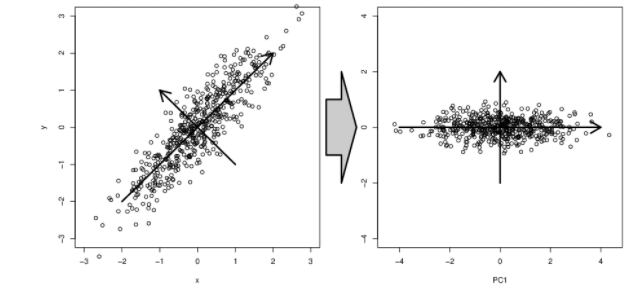
\includegraphics[width=0.6\linewidth]{S4.png}
		\caption{Przykład PCA}
	\end{figure}

	\item \textbf{ISOMAP}
	
	ISOMAP jest metodą, która w porównaniu do pozostałych zdecydowanie \textbf{lepiej radzi sobie z nieliniowymi danymi}. Jej celem jest znalezienie niskowymiarowej reprezentacji danych, w której \textbf{odległości rzeczywiste między elementami z próby są jak najbliższe tym z oryginalnej przestrzeni wysokowymiarowej}. \\
	
	Kroki metody ISOMAP wyglądają następująco:
	\begin{itemize}
		\item \textbf{Wyszukiwanie najbliższego sąsiada} - tworzony jest graf sąsiedztwa pomiędzy punktami w danych według zasady: jeżeli odległość między punktami jest mniejsza niż założona z góry odległość to tworzona jest krawędź pomiędzy tymi punktami.
		\item \textbf{Wyszukiwanie najkrótszej drogi} – dla każdej pary punktów znajdowana jest najkrótsza odległość pomiędzy tymi punktami na utworzonym w kroku pierwszym grafie.
		\item \textbf{Skalowanie} – stosowana jest metoda skalowania wielowymiarowego czyli technika przyjmująca na wejściu macierz odległości lub podobieństwa a następnie dąży do rozmieszczenia obiektów jako punktów w przestrzeni n-wymiarowej tak aby obiekty podobne do siebie znajdowały się bliżej.  Wynikiem tego etapu jest reprezentacja danych w mniejszym wymiarze. \\
	\end{itemize}

	\item \textbf{T-SNE}
	
	T-SNE czyli stochastyczna metoda porządkowania sąsiadów w oparciu o rozkład t. W porównaniu do PCA jest ona droga obliczeniowo i dla dużej ilości wymiarów jej wyliczenie może zająć nawet kilka godzin gdzie PCA zakończy się w ciągu kilku minut. Jest ona także techniką probabilistyczną przez co nawet dla dokładnie tych samych parametrów jej obliczenie wiele razy da za każdym razem inny wynik. \\
	
	Kroki tej metody wyglądają następująco:
	\begin{itemize}
		\item \textbf{Wyliczenie podobieństw wszystkich danych}
			\begin{figure}[H]
				\centering
				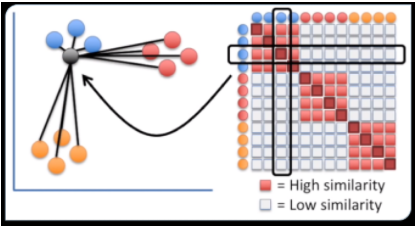
\includegraphics[width=0.5\linewidth]{S4_1.png}
			\end{figure}
		\item \textbf{Wyliczenie losowych podobieństw}
		\item \textbf{Odzwierciedlanie zestawów prawdopodobieństw w docelowej ilości wymiarów}
			\begin{figure}[H]
				\centering
				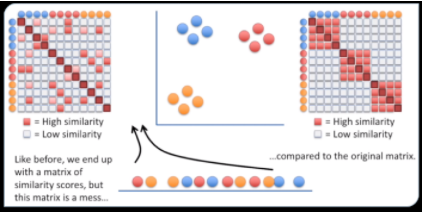
\includegraphics[width=0.5\linewidth]{S4_2.png}
			\end{figure}
	\end{itemize}
\end{itemize}
